%!TEX encoding = UTF-8 Unicode
\chapter{动态分析}
动态分析是需要样本中的代码在目标系统实际运行起来的分析方式。与静态分析相比,它能够获得更直观、更全面的结果。此外,对采用了代码混淆等对抗技术的样本,动态分析会是主要的手段。

与静态分析相比,动态分析的知识点比较杂,没有系统的基础知识,也需要更高的创造力和综合能力。

\section{运行环境}
\subsection{模拟器}
Android SDK提供了用于应用软件开发的Android模拟器\lstinline!emulator!\footnote{\url{http://developer.android.com/guide/developing/tools/emulator.html}}\index{emulator},是首选的运行环境。
\begin{figure}[htbp]
  \centering
  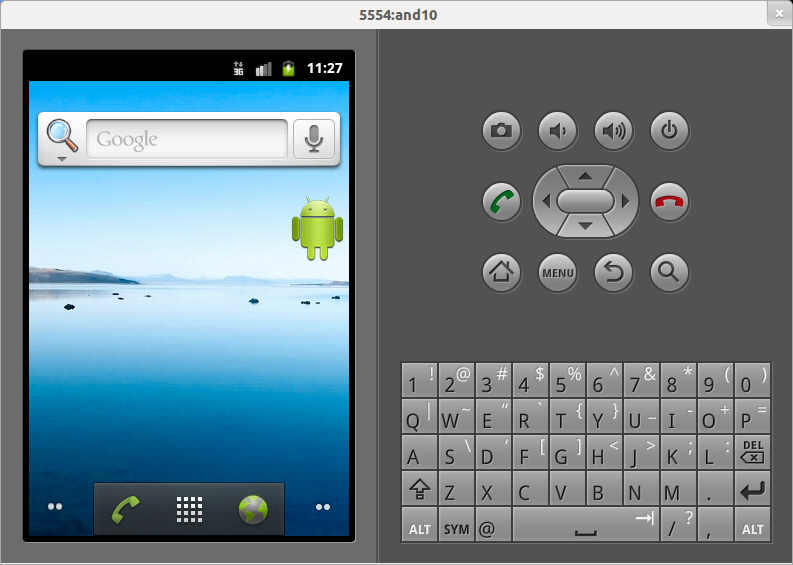
\includegraphics[width=14cm]{image/emulator.png}
  \caption{emulator模拟器}
\end{figure}

\lstinline!emulator!中模拟的Android系称为AVD(Android Virtual Device),由SDK中\lstinline!android!\footnote{\url{http://developer.android.com/guide/developing/tools/android.html}}\index{android}工具创建:
\begin{lstlisting}[language=bash, numbers=none]
 $ android create avd -n my_avd -t android-10
\end{lstlisting}

可以使用图形化的AVD Manager直接启动AVD,也可以使用\lstinline!emulator!直接启动。使用命令行参数可以手工指定一些高级选项,这在一些分析时可能会用上。这些参数如下:
\begin{itemize}
\item \lstinline!-avd!,必选参数,指定AVD的名字
\item \lstinline!-data!,手工指定一个data分区镜像文件
\item \lstinline!-ramdisk!,手工指定一个RAM镜像文件
\item \lstinline!-kernel!,手工指定一个内核文件
\item \lstinline!-system!,手工指定一个system分区镜像文件
\item \lstinline!-sdcard!,手工指定一个SD卡镜像文件,该文件可以用\lstinline!mksdcard!创建
\item \lstinline!-dns-server!,给出DNS服务器地址,可以指向自己搭建的DNS服务器,模拟样本依赖的服务器
\item \lstinline!-http-proxy!,当样本访问被墙的网址时,可以通过SSH隧道和本地HTTP端口转发
\item \lstinline!-debug!,打开或关闭指定的调试标签,让\lstinline!emulator!输出调试信息,可以使用\lstinline!emulator -help-debug-tags!察看有哪些标签
\end{itemize}
例如,\lstinline!droidbox!的启动命令行是:
\begin{lstlisting}[language=bash, numbers=none]
 $ emulator -avd droidbox -system system.img -ramdisk ramdisk.img -kernel zImage -prop dalvik.vm.execution-mode=int:portable
\end{lstlisting}

\lstinline!emulator!的不足之处是:
\begin{itemize}
\item 虽然可以模拟短信和通话,但并没有与真正的移动通信网络相连
\item 对依赖于ROM环境、依赖于特定手机型号的样本不起作用
\end{itemize}

\subsection{手机}
手机可以提供运行样本的真实环境,并且与移动通信网相连。主要缺点是成本较高。

推荐Google的Nexus S型号手机,原因包括:
\begin{itemize}
  \item 直接使用Android源码可以编译Nexus S系统镜像,自行修改的源码可以获得真实的运行环境,并且可以对该镜像做自由的修改,比如有root权限、可以修改启动配置等
  \item 诸如TaintDroid、AppFence等项目均提供了用于Nexus S的源码
  \item 可以在第一时间获得新版本系统,例如Android 4.0
  \item 综合性价比较高
\end{itemize}

\subsection{Android-x86}
Android-x86\footnote{\url{http://www.android-x86.org}}\index{Android-x86}提供了用于Intel x86处理器的Android系统镜像,可以将其安装到诸如VirtualBox和VMware WorkStation这样的虚拟机中。有研究称该项目系统的启动速度是\lstinline!emulator!中AVD启动速度的四分之一。

\section{设备管理}
\subsection{adb}
\lstinline!adb!是连接PC与设备(模拟器或手机)的主要工具,其用法在Android开发文档中有详细的说明\footnote{\url{http://developer.android.com/guide/developing/tools/adb.html}}。

它的功能包括:
\begin{itemize}
\item 提供了一个访问Android底层Linux系统的shell
\item 通过push和pull在PC和设备之间传输文件
\item 通过install和uninstall安装或卸载应用程序
\item 转发对Android系统的调试指令和数据
\item 通过logcat获取系统进程和应用程序输出的日志信息
\end{itemize}

\subsection{ddms}
SDK中的ddms提供了一个细粒度的可视化调试环境。
\section{网络分析}
\subsection{tcpdump}
为了捕获样本在运行期间产生的网络数据,需要对其抓包。主要工具是tcpdump。针对不同的场景,可以在三个不同的位置使用这一工具。
\subsubsection{模拟器}
模拟器emulator有一个没有公开的参数-tcpdump,在启动模拟器时,通过该参数指定一个本地文件路径,可以将模拟器运行期间产生的所有网络数据捕获到指定的pcap文件。
\subsubsection{Android系统}
有移植到Android底层的原生tcpdump工具,但其运行需要root权限。这一工具可以在模拟器中的系统里运行,但更多时候用于真实手机系统的抓包。
\subsubsection{PC网络}
当真实手机使用Wi-Fi通信,可以在无线网络或者其后端的物理网络抓包。
\subsection{wireshark}
对网络数据的分析一般使用wireshark这一传统的网络分析工具。最常用的功能是其filter。

\subsection{android proxy}
\section{行为模拟}
\subsection{am}

\subsection{DNS}

\subsection{telnet}
通过telnet可以与模拟器中的Android系统收发短信、拨打接听电话。
\subsection{openBTS}
对真实手机中的Android系统,可以通过架设一个OpenBTS系统来获取其发送短信、拨打电话的行为,并模拟任意的外部号码向其发送短信、拨打电话。

\section{行为跟踪}
\subsection{droidbox}
\subsection{LBE}

\section{调试}
\label{Sec:debug}
\subsection{apktool}
\subsection{AndBug}

\section{衍生文件}
